% ============================================================================ %
%
%           Šablona bakalářské/diplomové práce
%
% Autor:    Ing. Jozef Říha (2006-05-04), od té doby šablonu udržuje
%           Ing. Pavel Tomášek, Ph.D. (tomasek@utb.cz)
%
% Verze:    2021-05-04
%
% Kódování: UTF-8 (kontrolní řetězec: žluťoučký kůň úpěl ďábelšké ódy)
%
% Sazba:    pdflatex prace.tex && pdflatex prace.tex
%           (nutné dvakrát pro korektní vložení citací a jiných referencí),
%           v případě umístění literatury do externího bib souboru je třeba volat
%           pdflatex prace.tex && bibtex prace && pdflatex prace.tex && pdflatex prace.tex
%
% Tip:      Ve správně vysázeném českém textu by na konci řádku neměla zůstant
%           samotná jednopísmenná předložka či spojka. Na takové místo se vkládá
%           nezalomitelná mezera pomocí symbolu ~. Existuje program, který umí
%           zpracovat celý TeX dokument najednou podle českých konvencí:
%           http://petr.olsak.net/ftp/olsak/vlna/
%
% Pozor:    Vzhledem k požadovanému standardu PDF/A nesmí vložené obrázky 
%           obsahovat alfa kanál (průhlednost).
%
% ============================================================================ %


\documentclass[a4paper,12pt]{article}

% Definice vzhledu a nastavení se načítá z následujícího souboru (netřeba editovat)
% ============================================================================ %
% Tento dokument není zpravidla třeba editovat,
% obsahuje nastavení balíčků, vzhledu, stylů.
%
% Kódování: UTF-8 (žluťoučký kůň úpěl ďábelšké ódy)
% ============================================================================ %


% ============================================================================ %
% BALÍČKY

%\usepackage[czech,english]{babel} % volba při kompilaci latexem (vyžaduje texlive-lang), zakomentovano, nastavovanu prikazem \nastavjazyk
\usepackage[T1]{fontenc}% definice vnitřního kódování
\usepackage[utf8x]{inputenc} % slouží pro definici kódování (při problémech zkusit zaměnit utf8x za utf8)
\usepackage{color}		% umožňuje použití barev
\usepackage{graphicx}	% rozšíření práce s grafikou
\usepackage{amsmath}	% balíček pro pokročilejší matematiku
\usepackage{fancyhdr}	% detailnější nastavení záhlaví a zápatí
\usepackage{tocloft}	% umožňuje pohodlné nastavení vzhledu obsahu, seznamu tabulek či obrázků
\usepackage{textcase}	% změna VeLiKoStI PíSmA
\usepackage{ifthen} 	% balíček umožňující skladby if, then -- využijeme při definici nadpisů
\usepackage{setspace}	% balíček umožňující nastavit řádkování na 1, 1.5, 2
\usepackage{ccaption}	% vylepšení práce s popisky obrázků či tabulek
\usepackage{sectsty}	% pro nastavení vzhledu nadpisů
\usepackage[srcstyle=leftnumhang,linenumbersep={\ }]{examplep} % pokročilejší sazba programového kódu
\usepackage{url}		% balíček pro vysázení internetové adresy stylem verbatim s vylepšeným řádkovým zlomem
\usepackage{afterpage}
%\usepackage{layout}	% zobrazí nastavení tiskového zrcadla (příkaz \layout)
%\usepackage{times}		% balíček pro použití fontu times
%\usepackage{verbatim}	% vysází text bez formátování, tak jak je zapsán v souboru
%\usepackage{indentfirst} % definuje odsazení prvního řádku odstavce
%\usepackage{makeidx}	% vytvoří rejstřík
\usepackage[pdftex,pdfa,hidelinks,breaklinks]{hyperref}	% vytváří křížové odkazy
%\usepackage{multicol}	% vícesloupcová sazba
%\usepackage{flafter}	% zajistí, aby se plovoucí objekty objevovali až za jejich umístěním v textu
\usepackage{chngcntr}	% Umožňuje změnu nastavení číslování obrázků, tabulek i rovnic
\usepackage{etoolbox}	% Tool-box for LaTeX programmers
\usepackage[labelsep=space,tableposition=bottom,justification=centering]{caption} % Přenastavení popisků u figur a tabulek
\usepackage{xmpincl}	% Pro aplikaci standardu PDF/A
\usepackage{hyperxmp}	% Pro aplikaci standardu PDF/A
\usepackage[final]{pdfpages}

%\pdfminorversion=4
%\pdfobjcompresslevel=0


% ---------------------------------------------------------------------------- %

% NASTAVENÍ TISKOVÉHO ZRCADLA

\newcommand{\valueTextHeight}{242mm}	% výška tiskového zrcadla
\newcommand{\valueTextWidth}{155mm}	% šířka tiskového zrcadla
\newcommand{\valueVOffset}{-1.61cm}	% vertikální posunutí tiskového zrcadla
\newcommand{\valueSideMargin}{0.96cm}	% levý okraj
\newcommand{\valueHeadHeight}{0.6cm}	% záhlaví
\newcommand{\valueHeadSep}{1cm}	% záhlaví

\textheight=\valueTextHeight
\textwidth=\valueTextWidth
\voffset=\valueVOffset
%\voffset=-1in
%\topmargin=-2.9cm

\oddsidemargin=\valueSideMargin
\evensidemargin=\valueSideMargin

\headheight=\valueHeadHeight
\headsep=\valueHeadSep

% nastavení zápatí
\footskip=1ex
\cfoot{}
% "vypnout" poznámky na okrajích
\marginparpush=0mm
\marginparwidth=0mm
\marginparsep=0mm

\pagestyle{fancy}

% Nastavení obalujících okrajů okolo popisků figur a tabulek
\captionsetup[figure]{aboveskip=5pt}
\captionsetup[figure]{belowskip=0pt}
\captionsetup[table]{aboveskip=0pt}
\captionsetup[table]{belowskip=5pt}


% ============================================================================ %
% NASTAVENÍ PÍSMA, ODSTAVCE, ROVNIC, POZNÁMEK

\parindent=0em				% velikost odstavcové zarážky na nulu
\def\thefootnote{\arabic{footnote})}	% poznámka pod čarou se závorkou
\onehalfspacing % nastavím řádkování tímto způsobem nebo \renewcommand{\baselinestretch}{1.5} ??
\setlength{\parskip}{3pt}		% vertikální mezera mezi nadpisy
%\def\label#1{{\sf ! #1 ! }}		% možnost zobrazení všech \label{}


% ============================================================================ %
% NASTAVENÍ ČÍTAČŮ

\setcounter{tocdepth}{3} % do obsahu se ukládají pouze první dvě úrovně kapitol


% ============================================================================ %
% PDF/A STANDARD

% http://www.mathstat.dal.ca/~selinger/pdfa/
% https://blog.zhaw.ch/icclab/creating-pdfa-documents-for-long-term-archiving/
% http://support.river-valley.com/wiki/index.php?title=Generating_PDF/A_compliant_PDFs_from_pdftex

% Prerequisites: pdflatex, hyperref, xmpincl
% pdfTeX at least in version 1.40.15 (in Linux add repository ppa:jonathonf/texlive, update and upgrade texlive-full)
%
% Validator: http://pdfa.k.utb.cz:8080/ https://www.pdf-online.com/osa/validate.aspx

% \convertDate converts D:20080419103507+02'00' to 2008-04-19T10:35:07+02:00
\def\convertDate{%
	\getYear
}
{\catcode`\D=12
 \gdef\getYear D:#1#2#3#4{\edef\xYear{#1#2#3#4}\getMonth}
}
\def\getMonth#1#2{\edef\xMonth{#1#2}\getDay}
\def\getDay#1#2{\edef\xDay{#1#2}\getHour}
\def\getHour#1#2{\edef\xHour{#1#2}\getMin}
\def\getMin#1#2{\edef\xMin{#1#2}\getSec}
\def\getSec#1#2{\edef\xSec{#1#2}\getTZh}
\def\getTZh +#1#2{\edef\xTZh{#1#2}\getTZm}
\def\getTZm '#1#2'{%
	\edef\xTZm{#1#2}%
	\edef\convDate{\xYear-\xMonth-\xDay T\xHour:\xMin:\xSec+\xTZh:\xTZm}%
}
\expandafter\convertDate\pdfcreationdate

\pdfminorversion 4

\immediate\pdfobj stream attr{/N 3} file{graphics/sRGBIEC1966-2.1.icm}
\pdfcatalog{%
	/OutputIntents [ <<
	/Type /OutputIntent
	/S/GTS_PDFA1
	/DestOutputProfile \the\pdflastobj\space 0 R
	/OutputConditionIdentifier (sRGB IEC61966-2.1)
	/Info(sRGB IEC61966-2.1)
 >> ]
}

\providecommand{\xmpOrg}{Tomas Bata University in Zlín, Czech Republic}
\providecommand{\xmpProducer}{}
\providecommand{\xmpDoi}{}
\providecommand{\xmpJournalnumber}{}
\providecommand{\xmpVolume}{}
\providecommand{\xmpIssue}{}
\providecommand{\xmpCoverDisplayDate}{}
\providecommand{\xmpCoverDate}{}
\providecommand{\xmpJournaltitle}{}
\providecommand{\xmpFirstpage}{}
\providecommand{\xmpLastpage}{}
\providecommand{\xmpAuthoritativeDomain}{}
\providecommand{\xmpCreatorTool}{}%pdfTeX

\newcommand{\aplikujpdfa}{
	\ifczech
		\providecommand{\xmpTitle}{\nazevcz}
		\providecommand{\xmpAuthor}{\autor}
		\providecommand{\xmpKeywords}{\klicovaslovacz}
		\hypersetup{
			pdftitle={\nazevcz},
			pdfauthor={\autor},
			pdfsubject={\abstraktcz},
			pdfkeywords={\klicovaslovacz},
			%pdfproducer={pdfTeX-1.40.20},
			pdflang=la,
			pdfapart=3,
			pdfaconformance=B,
			pdflang={cz}
		}
	\else \ifenglish
		\providecommand{\xmpTitle}{\nazeven}
		\providecommand{\xmpAuthor}{\autor}
		\providecommand{\xmpKeywords}{\klicovaslovaen}
		\hypersetup{
			pdftitle={\nazeven},
			pdfauthor={\autor},
			pdfsubject={\abstrakten},
			pdfkeywords={\klicovaslovaen},
			%pdfproducer={pdfTeX-1.40.20},
			pdflang=la,
			pdfapart=3,
			pdfaconformance=B,
			pdflang={en}
		}
	\fi \fi
	
	\makeatletter
	\includexmp{tex/pdfa-1b}
	\makeatother
}


% ============================================================================ %
% UŽIVATELSKÉ STYLY

% Styl nn = nečíslovaný nadpis (je vysázený v obsahu)
\def\nn#1{\clearpage\phantomsection\addcontentsline{toc}{section}{#1}\section*{\MakeTextUppercase{#1}}}

% Styl nm = nečíslovaný nadpis (není vysázený v obsahu)
\def\nm#1{\clearpage\section*{\MakeTextUppercase{#1}}}

% Styl ns = nečíslovaný nadpis na stejné stránce (není vysázený v obsahu)
\def\nns#1{\section*{\MakeTextUppercase{#1}}}

% Styl n{ur}{nadp} pro nadpisy, kde ur je číslo úrovně a nadp je text nadpisu
\def\n#1#2{
	
	\ifthenelse{#1=1}{
		\sectionfont{\normalsize\MakeUppercase}
		\clearpage\section{#2}
		\sectionfont{\normalsize}
		}{
		\ifthenelse{#1=2}{\subsection{#2}}{
			\ifthenelse{#1=3}{\subsubsection{#2}}{\paragraph{\itshape\bfseries{#2}}
}}}}

% Styl pro obrázky
% \obr{popisek}{label}{rozměr (0.0 - 1.0)}{soubor}
\def\obr#1#2#3#4{
	\begin{figure}[h]
		\centering
		\includegraphics[width=#3\linewidth]{#4}
		%\captionwidth{#3\linewidth}
		%\changecaptionwidth
		\captionsetup{width=#3\linewidth}
		\caption{#1}
		\label{#2}
	\end{figure}
}

% Styl pro tabulky
% \tab{popisek}{label}{rozměr (0.0 - 1.0)}{definice sloupců}{obsah} 
\def\tab#1#2#3#4#5{
	\begin{table}[h]
		%\captionwidth{#3\linewidth}
		%\changecaptionwidth
		\captionsetup{width=#3\linewidth}
		\caption{#1}
		\label{#2}
		\centering
		\begin{tabular}{#4}
			#5
		\end{tabular}
	\end{table}
}

% Styl pro tabulky v příloze
% \tabpri{popisek}{definice sloupců}{data tabulky}
\def\tabpri#1#2#3{
	\begin{table}[h]
	\begin{center}
	#1
	\end{center}
	\begin{center}
	\begin{tabular}{#2}
	#3
	\end{tabular}
	\end{center}
	\end{table}
}
	
% Styl pro tabulky z MS Excelu exportované do EPS
% \extab{popisek}{rozměr (0.0 - 1.0)}{soubor}
\def\extab#1#2#3{
	\begin{table}
	%\captionwidth{#2\linewidth}
	%\changecaptionwidth
	\captionsetup{width=#2\linewidth}
	\caption{#1}
	\begin{center}
	\includegraphics[width=#2\linewidth]{#3}
	\end{center}
	\end{table}
}

% Styl pro rovnice
% \rov[klíčové slovo]{rovnice}
\newcommand{\rov}[2][chybejici rovnice]{
	\begin{equation}
	#2
	\label{#1}
	\end{equation}
}
	
% Příkaz pro vysázení seznamu obrázků
\def\seznamobr{
	\clearpage
	\phantomsection
	\ifczech
		\addcontentsline{toc}{section}{Seznam obrázků}
	\else \ifenglish
		\addcontentsline{toc}{section}{List of Figures}
	\fi \fi
	\listoffigures
	\clearpage
}

% Příkaz pro vysázení seznamu tabulek
\def\seznamtab{
	\clearpage
	\phantomsection
	\ifczech
		\addcontentsline{toc}{section}{Seznam tabulek}
	\else \ifenglish
		\addcontentsline{toc}{section}{List of Tables}
	\fi \fi
	\listoftables
	\clearpage
}

\newcommand{\OdsazovaniOdstavcuStart}[0]{
	\ifenglish
		\setlength{\parskip}{5mm} % English indentation of paragraphs
	\else \ifczech
		\setlength{\parindent}{5mm} % Czech indentation of paragraphs
	\fi \fi
}

\newcommand{\OdsazovaniOdstavcuStop}[0]{
	\ifenglish
		\setlength{\parskip}{0mm} % English indentation of paragraphs
	\else \ifczech
		\setlength{\parindent}{0mm} % Czech indentation of paragraphs
	\fi \fi
}

% Příkaz pro vysázení seznamu literatury
\newcommand{\seznamlit}[1]{
	\clearpage
	\phantomsection
	\ifczech
		\addcontentsline{toc}{section}{Seznam použité literatury}
	\else \ifenglish
		\addcontentsline{toc}{section}{References}
	\fi \fi
	\begin{thebibliography}{99}
	#1
	\end{thebibliography}
}

\newcommand{\seznamlitbib}{
	\bibliographystyle{\ifenglish tex/czechiso-en\else\ifczech tex/czechiso-cz\fi\fi} % Respects the norm of ČSN ISO 690
	\newpage
	\clearpage
	%\cleardoublepage
	\phantomsection
	\addcontentsline{toc}{section}{\ifenglish References \else \ifczech Seznam použité literatury \fi \fi}
	\bibliography{tex/literatura}
}

% Příkaz pro přípravu seznamu použitých zkratek a symbolů
\newcommand{\seznamzkr}{
	\ifczech
		\nn{Seznam použitých symbolů a zkratek}
	\else \ifenglish
		\nn{List of Abbreviations}
	\fi \fi
}

% Příkaz \cast jako alternativa k \part
\def\cast#1{
	\clearpage
	\part{#1}
}

% Příkaz \obsah vysází obsah v daném místě
\def\obsah{
	\deaktivujZahlavi
	\clearpage
	\thispagestyle{empty}
	\tableofcontents
	\clearpage
	\pagestyle{fancy}
	\aktivujZahlavi
}

% Zkrácení stylu \textbf na \b
\def\b#1{
	\textbf{#1}
}

% \bi = tučná kurzíva
\newcommand{\bi}[1]{\textbf{\textit{#1}}}

% \it = kurzíva
\renewcommand{\it}[1]{\textit{#1}}

% Nastaveni nezobrazovani zahlavi dokumentu
\newcommand{\deaktivujZahlavi}{
	\lhead{}
	\rhead{}
	\renewcommand{\headrulewidth}{0pt}
}

\newcommand{\zadani}{
	% \clearpage
	% \thispagestyle{empty}
	% \voffset=\valueVOffset\evensidemargin=\valueSideMargin\oddsidemargin=\valueSideMargin\headsep=\valueHeadSep\headheight=\valueHeadHeight\setlength{\parskip}{3pt}\textheight=\valueTextHeight\textwidth=\valueTextWidth
	% *** Nascanované zadání, strana 1 ***
	
	% \clearpage
	% \thispagestyle{empty}
	% *** Nascanované zadání, strana 2 ***
	\voffset=\valueVOffset\evensidemargin=\valueSideMargin\oddsidemargin=\valueSideMargin\headsep=\valueHeadSep\headheight=\valueHeadHeight\setlength{\parskip}{3pt}\textheight=\valueTextHeight\textwidth=\valueTextWidth
	\includepdf[pages=-]{zadani.pdf}
	%\includepdf[pages=1-2, pagecommand={}, trim=1cm 2cm 1cm 2cm, clip]{~/School/Thesis/Thesis/tex/zadani.pdf}
}

% Nastaveni zobrazovani zahlavi dokumentu
\newcommand{\aktivujZahlavi}{
	\renewcommand{\headrulewidth}{1pt}
	\rhead{\thepage}
	
	\ifczech
		\lhead{\b{UTB ve Zlíně, \ifthenelse{\equal{\fakulta}{FAI}}{Fakulta aplikované informatiky}{\ifthenelse{\equal{\fakulta}{FAME}}{Fakulta managementu a ekonomiky}{\ifthenelse{\equal{\fakulta}{FHS}}{Fakulta humanitních studií}{\ifthenelse{\equal{\fakulta}{FLKR}}{Fakulta logistiky a krizového řízení}{\ifthenelse{\equal{\fakulta}{FMK}}{Fakulta multimediálních komunikací}{\ifthenelse{\equal{\fakulta}{FT}}{Fakulta technologická}{\ifthenelse{\equal{\fakulta}{UNI}}{Univerzitní institut}{}}}}}}}}}
	\else \ifenglish
		\lhead{\b{TBU in Zlín, \ifthenelse{\equal{\fakulta}{FAI}}{Faculty of Applied Informatics}{\ifthenelse{\equal{\fakulta}{FAME}}{Faculty of Management and Economics}{\ifthenelse{\equal{\fakulta}{FHS}}{Faculty of Humanities}{\ifthenelse{\equal{\fakulta}{FLKR}}{Faculty of Logistics and Crisis Management}{\ifthenelse{\equal{\fakulta}{FMK}}{Faculty of Multimedia Communications}{\ifthenelse{\equal{\fakulta}{FT}}{Faculty of Technology}{\ifthenelse{\equal{\fakulta}{UNI}}{University Institute}{}}}}}}}}}
	\fi \fi
}

% Příkaz \logopracerok vloží na dané místo logo fakulty, typ práce a rok
\newcommand{\logopracerok}{
	\ifczech
		\iffai	\put(82.2,-223.3){\makebox(84,16.4){
\includegraphics[width=90mm]{graphics/logo/fai_logo_cz.png}}} \fi
		\iffame	\put(82.2,-223.3){\makebox(84,16.4){
\includegraphics[width=90mm]{graphics/logo/fame_logo_cz.png}}} \fi
		\iffhs	\put(82.2,-223.3){\makebox(84,16.4){
\includegraphics[width=90mm]{graphics/logo/fhs_logo_cz.png}}} \fi
		\ifflkr	\put(82.2,-223.3){\makebox(84,16.4){
\includegraphics[width=90mm]{graphics/logo/flkr_logo_cz.png}}} \fi
		\iffmk	\put(82.2,-223.3){\makebox(84,16.4){
\includegraphics[width=90mm]{graphics/logo/fmk_logo_cz.png}}} \fi
		\ifft	\put(82.2,-223.3){\makebox(84,16.4){
\includegraphics[width=90mm]{graphics/logo/ft_logo_cz.png}}} \fi
		\ifuni	\put(82.2,-223.3){\makebox(84,16.4){
\includegraphics[width=90mm]{graphics/logo/uni_logo_cz.png}}} \fi
	\else \ifenglish
		\iffai	\put(82.2,-223.3){\makebox(84,16.4){
\includegraphics[width=90mm]{graphics/logo/fai_logo_en.png}}} \fi
		\iffame	\put(82.2,-223.3){\makebox(84,16.4){
\includegraphics[width=90mm]{graphics/logo/fame_logo_en.png}}} \fi
		\iffhs	\put(82.2,-223.3){\makebox(84,16.4){
\includegraphics[width=90mm]{graphics/logo/fhs_logo_en.png}}} \fi
		\ifflkr	\put(82.2,-223.3){\makebox(84,16.4){
\includegraphics[width=90mm]{graphics/logo/flkr_logo_en.png}}} \fi
		\iffmk	\put(82.2,-223.3){\makebox(84,16.4){
\includegraphics[width=90mm]{graphics/logo/fmk_logo_en.png}}} \fi
		\ifft	\put(82.2,-223.3){\makebox(84,16.4){
\includegraphics[width=90mm]{graphics/logo/ft_logo_en.png}}} \fi
		\ifuni	\put(82.2,-223.3){\makebox(84,16.4){
\includegraphics[width=90mm]{graphics/logo/uni_logo_en.png}}} \fi
	\fi \fi
	\put(0,-205){\linethickness{1pt}\line(1,0){170}}
	\ifczech
		\ifbp \put(4,-215){\makebox(69.5,4.5)[l]{\noindent\fontsize{16}{1}\usefont{OT1}{phv}{m}{n}Bakalářská práce}} \fi
		\ifdp \put(4,-215){\makebox(69.5,4.5)[l]{\noindent\fontsize{16}{1}\usefont{OT1}{phv}{m}{n}Diplomová práce}} \fi
	\else \ifenglish
		\ifbp \put(4,-215){\makebox(69.5,4.5)[l]{\noindent\fontsize{16}{1}\usefont{OT1}{phv}{m}{n}Bachelor's thesis}} \fi
		\ifdp \put(4,-215){\makebox(69.5,4.5)[l]{\noindent\fontsize{16}{1}\usefont{OT1}{phv}{m}{n}Master's thesis}} \fi
	\fi \fi
	\put(4,-220){\makebox(69.5,4.5)[l]{\noindent\fontsize{16}{1}\usefont{OT1}{phv}{m}{n}\rok}}
	\put(0,-225){\linethickness{1pt}\line(1,0){170}}
	\put(75,-223.3){\linethickness{1pt}\line(0,1){16.4}}
}

% Úvodní stránka s logem fakulty
\newcommand{\titulnistrana}{
	\thispagestyle{empty}
	\voffset=-2.01cm\evensidemargin=0pt\oddsidemargin=0cm\parindent=0pt\headsep=0pt\headheight=0pt\parskip=0pt\textheight=272mm\textwidth=200mm
	\renewcommand{\baselinestretch}{0}
	
	\setlength{\unitlength}{1mm}
	\begin{picture}(-10,8)
		\ifczech
			% Nazev prace
			%\put(0,-100){\makebox(170,50){\fontsize{24}{1}\usefont{OT1}{phv}{b}{n}#1}}
			%		\put(0,-100){\makebox(170,50){\protect\parbox{0.8\textwidth}{\protect\centering\fontsize{24}{1}\usefont{OT1}{phv}{b}{n}#1}}}
			
			% Vyreseno odradkovani
			\put(0,-100){\makebox(170,50){\protect\parbox{0.8\textwidth}{\protect\centering\setstretch{2.0}\usefont{OT1}{phv}{b}{n}{\Huge\nazevcz}}}}
			
			% Jmeno autora
			\put(0,-135){\makebox(170,25){\fontsize{20}{1}\usefont{OT1}{phv}{m}{n}\autor}}
		\else \ifenglish
			% Nazev prace
			%\put(0,-100){\makebox(170,50){\fontsize{24}{1}\usefont{OT1}{phv}{b}{n}#1}}
			%\put(0,-95){\makebox(170,50){\protect\parbox{0.8\textwidth}{\protect\centering\fontsize{24}{1}\usefont{OT1}{phv}{b}{n}#1}}}
			%\put(0,-88)%toto bylo pouzito v pripade zobrazeni nazvu ve dvou jazycich
			\put(0,-100){\makebox(170,50){\protect\parbox{0.8\textwidth}{\protect\centering\setstretch{2.0}\usefont{OT1}{phv}{b}{n}{\Huge\nazeven}}}}
	
			%\put(0,-111){\makebox(170,50){\fontsize{20}{1}\usefont{OT1}{phv}{m}{n}#1}}
			%\put(0,-116){\makebox(170,50){\protect\parbox{0.8\textwidth}{\protect\centering\fontsize{20}{1}\usefont{OT1}{phv}{m}{n}#2}}}
			%\put(0,-115){\makebox(170,50){\protect\parbox{0.8\textwidth}{\protect\centering\setstretch{1.5}\usefont{OT1}{phv}{m}{n}{\Large\nazevcz}}}}
			
			% Jmeno autora
			\put(0,-135){\makebox(170,25){\fontsize{20}{1}\usefont{OT1}{phv}{m}{n}\autor}}
		\fi \fi
		\logopracerok
	\end{picture}
}


% Strana s abstraktem a klíčovými slovy v češtině a angličtině
\newcommand{\abstraktaklicovaslova}{
	\clearpage
	\thispagestyle{empty}
	\nm{Abstrakt}
	\abstraktcz
	
	\vspace{1cm}
	Klíčová slova: \klicovaslovacz
	
	\vspace{3cm}
	
	\nns{Abstract}
	\abstrakten
	
	\vspace{1cm}
	Keywords: \klicovaslovaen
}


% ============================================================================ %
% NASTAVENÍ ZOBRAZENÍ PŘÍLOH -- SEZNAM, ČÍSLOVÁNÍ, VLASTNÍ STYL

\makeatletter % tímto příkazem dávám najevo, že budu editovat přímo příkazy ze šablony

% definice seznamu příloh - příkaz \listofappendices
\def\listofappendices{%
	\newpage
	\phantomsection
	\setcounter{section}{0}
	\ifczech
		\addcontentsline{toc}{section}{Seznam příloh}
		\@restonecolfalse\if@twocolumn\@restonecoltrue\onecolumn\fi
		\section*{SEZNAM PŘÍLOH}
	\else \ifenglish
		\addcontentsline{toc}{section}{List of Appendices}
		\@restonecolfalse\if@twocolumn\@restonecoltrue\onecolumn\fi
		\section*{LIST OF APPENDICES}
	\fi \fi
	\@mkboth{LIST OF APPENDICES}{LIST OF APPENDICES}
	\@starttoc{loa}\if@restonecol\twocolumn\fi
	\pagestyle{empty}
	\thispagestyle{fancy}
}

\def\ext@appendix{loa}
\def\tocname{loa}

% definice příkazu \priloha{nazev prilohy} pro vložení nové přílohy
\newcommand{\priloha}[1]{
	\clearpage
	\refstepcounter{section}
	%\voffset=-3cm % vertikalni posun
	\addtocontents{loa}{\protect\makebox[1.5cm][l]{\ifczech P\else \ifenglish A\fi\fi\ \@Roman\c@section.} #1\newline}
	\ifczech
		{\bf PŘÍLOHA \ifczech P\else \ifenglish A\fi\fi\ \@Roman\c@section. \MakeTextUppercase{#1}}
	\else \ifenglish
		{\bf APPENDIX \ifczech P\else \ifenglish A\fi\fi\ \@Roman\c@section. \MakeTextUppercase{#1}}
	\fi \fi
	\par
}

% ============================================================================ %
% OBSAH: NASTAVENÍ VELKÝCH PÍSMEN PRO NÁZVY SEKCÍ A HLAVNÍCH NADPISŮ

\let\oldcontentsline\contentsline
\def\contentsline#1#2{%
	\expandafter\ifx\csname l@#1\endcsname\l@section
		\expandafter\@firstoftwo
	\else
		\expandafter\@secondoftwo
	\fi
	{%
		\oldcontentsline{#1}{\MakeTextUppercase{#2}}%
	}{%
		\oldcontentsline{#1}{#2}%
	}%
}

\def\@part[#1]#2{
	\ifnum \c@secnumdepth >\m@ne
		\refstepcounter{part}
		\addcontentsline{toc}{section}{\protect\texorpdfstring{\makebox[0.85cm]{\thepart\hfill} #1}{\thepart\ #1}}
	\else
		\addcontentsline{toc}{section}{#1}
	\fi
	{\parindent \z@ \raggedright
	\interlinepenalty \@M
	\clearpage
	\normalfont
	\ifnum \c@secnumdepth >\m@ne
		\Large\bfseries
		\nobreak
	\fi
	\vspace*{9cm}
	\center\huge \bfseries\thepart. \MakeTextUppercase{#2}
	\markboth{}{}\par}
	\nobreak
	\clearpage
	\@afterheading
}


% ============================================================================ %
% NASTAVENÍ FORMÁTU ČÍSLOVÁNÍ OBRÁZKŮ A TABULEK

\def\thefigure{\arabic{figure}}	% číslování obrázků typu (y)
\def\thetable{\arabic{table}}	% číslování tabulek typu (y)
\captiondelim{. } % změníme dvoutečku za Obr/Tab za tečku

% Nastavení číslování obrázků, tabulek i rovnic do formátu <číslo kapitoly>.<pořadové číslo>
\counterwithin{figure}{section}
\counterwithin{table}{section}
\counterwithin{equation}{section}

% Odsazeni popisku v seznamu obrazku a tabulek
\patchcmd{\@caption}{\csname the#1\endcsname}{\csname fnum@#1\endcsname}{}{}
%{\renewcommand*\numberline[1]{Fig. \,#1\space}}
%\renewcommand*\l@figure{\@dottedtocline{1}{0em}{5.0em}}
%\renewcommand*\l@table{\@dottedtocline{1}{0em}{5.0em}}

% Vynulování čítačů
\@addtoreset{table}{section}
\@addtoreset{figure}{section}
\@addtoreset{footnote}{section}

\makeatother % a to je ukončení \makeatletter


% ============================================================================ %
% ÚPRAVA VZHLEDU OBSAHU, SEZNAMU OBRÁZKŮ A TABULEK

% nastavení vertikální mezery před stylem část, nadpis 1--3
\setlength{\cftbeforepartskip}{3pt}
\setlength{\cftbeforesecskip}{3pt}
\setlength{\cftbeforesubsecskip}{3pt}
\setlength{\cftbeforesubsubsecskip}{0cm}

% odsazení zleva pro styl část, nadpis 1--3
\setlength{\cftpartindent}{0cm}
\setlength{\cftsecindent}{0cm}
\setlength{\cftsubsecindent}{0cm}
\setlength{\cftsubsubsecindent}{0cm}

% nastavení fontu pro styl část, nadpis 1--3
\renewcommand{\cftpartfont}{\small\bfseries}
\renewcommand{\cftsecfont}{\small\bfseries}
\renewcommand{\cftsubsecfont}{\scshape}
\renewcommand{\cftsubsubsecfont}{}

% odsazení čísla a textu titulku pro styl část, nadpis 1--3
\cftsetindents{part}{0cm}{1cm}
\cftsetindents{sec}{0cm}{1cm}
\cftsetindents{subsec}{0.5cm}{1.25cm}
\cftsetindents{subsubsec}{1cm}{1.5cm}
\cftsetindents{fig}{0cm}{1.5cm}
\cftsetindents{tab}{0cm}{1.5cm}

% nastavení vodící čáry pro styl část, nadpis 1--3, obrázky a tabulky
\renewcommand{\cftdot}{\ensuremath{.}} % tímto příkazem lze změnit vodící tečky v obsahu na jiný znak
\renewcommand{\cftpartleader}{\cftdotfill{0.3}}
\renewcommand{\cftsecleader}{\cftdotfill{0.3}}
\renewcommand{\cftsubsecleader}{\cftdotfill{0.3}}
\renewcommand{\cftsubsubsecleader}{\cftdotfill{0.3}}
\renewcommand{\cftfigleader}{\cftdotfill{0.3}}
\renewcommand{\cfttableader}{\cftdotfill{0.3}}

% změna fontu pro text "Obsah", "Seznam obrázků" a "Seznam tabulek"
\renewcommand{\cfttoctitlefont}{\normalsize\bfseries\thispagestyle{empty}}
\renewcommand{\cftloftitlefont}{\normalsize\bfseries\thispagestyle{fancy}}
\renewcommand{\cftlottitlefont}{\normalsize\bfseries\thispagestyle{fancy}}

\renewcommand{\cfttabpresnum}{Tab. }
\renewcommand{\cftfigaftersnum}{.}
\renewcommand{\cfttabaftersnum}{.}
\setlength{\cftfignumwidth}{5em}
\setlength{\cfttabnumwidth}{5em}


% ============================================================================ %
% NASTAVENÍ FONTU PRO NADPISY

\sectionfont{\normalsize}
\subsectionfont{\normalsize\bfseries}
\subsubsectionfont{\small\bfseries}
\paragraphfont{\small\bf}

% definice nového stylu \comment -- komentář k šabloně
\newcommand{\comment}[1]{\color{red}#1\color{black}}


% ============================================================================ %
% VSTUPY

% Nastaveni a kontrola fakulty
\newcommand{\nastavfakultu}[1]{
	\newcommand{\fakulta}{#1}
	\newif\iffai	\let\iffai\iffalse
	\newif\iffame	\let\iffame\iffalse
	\newif\iffhs	\let\iffhs\iffalse
	\newif\ifflkr	\let\ifflkr\iffalse
	\newif\iffmk	\let\iffmk\iffalse
	\newif\ifft		\let\ifft\iffalse
	\newif\ifuni	\let\ifuni\iffalse
	
	\ifthenelse{\equal{#1}{FAI}}{\let\iffai\iftrue}{}
	\ifthenelse{\equal{#1}{FAME}}{\let\iffame\iftrue}{}
	\ifthenelse{\equal{#1}{FHS}}{\let\iffhs\iftrue}{}
	\ifthenelse{\equal{#1}{FLKR}}{\let\ifflkr\iftrue}{}
	\ifthenelse{\equal{#1}{FMK}}{\let\iffmk\iftrue}{}
	\ifthenelse{\equal{#1}{FT}}{\let\ifft\iftrue}{}
	\ifthenelse{\equal{#1}{UNI}}{\let\ifuni\iftrue}{}
	
	\iffai \else \iffame \else \iffhs \else \ifflkr \else \iffmk \else \ifft \else \ifuni \else
		\errmessage{Chyba nastaveni fakulty}
	\fi \fi \fi \fi \fi \fi \fi
}

% Nastaveni a kontrola typu prace
\newcommand{\nastavtyp}[1]{
	\newcommand{\typ}{#1}
	
	\newif\ifbp \let\ifbp\iffalse
	\newif\ifdp \let\ifdp\iffalse
	
	\ifthenelse{\equal{#1}{BP}}{\let\ifbp\iftrue}{}
	\ifthenelse{\equal{#1}{DP}}{\let\ifdp\iftrue}{}
	
	\ifbp \else \ifdp \else
		\errmessage{Chyba nastaveni typu prace}
	\fi \fi
}

% Nastaveni roku
\newcommand{\nastavrok}[1]{
	\newcommand{\rok}{#1}
}

% Nastaveni jmena
\newcommand{\nastavautora}[1]{
	\newcommand{\autor}{#1}
}

% Nastaveni nazvu
\newcommand{\nastavnazevcz}[1]{
	\newcommand{\nazevcz}{#1}
}
\newcommand{\nastavnazeven}[1]{
	\newcommand{\nazeven}{#1}
}

% Nastaveni abstraktu
\newcommand{\nastavabstraktcz}[1]{
	\newcommand{\abstraktcz}{#1}
}
\newcommand{\nastavabstrakten}[1]{
	\newcommand{\abstrakten}{#1}
}

% Nastaveni klicovych slov
\newcommand{\nastavklicovaslovacz}[1]{
	\newcommand{\klicovaslovacz}{#1}
}
\newcommand{\nastavklicovaslovaen}[1]{
	\newcommand{\klicovaslovaen}{#1}
}

% Nastaveni a kontrola jazyka
\newcommand{\nastavjazyk}[1]{
	\newcommand{\jazyk}{#1}
	
	\newif\ifczech		\let\ifczech\iffalse
	\newif\ifenglish	\let\ifenglish\iffalse
	
	\ifthenelse{\equal{#1}{CZ}}{\let\ifczech\iftrue}{}
	\ifthenelse{\equal{#1}{EN}}{\let\ifenglish\iftrue}{}
	
	\ifczech \else \ifenglish \else
		\errmessage{Chyba nastaveni jazyka}
	\fi \fi
	
	\ifczech
		\usepackage[czech]{babel}
		% Vlastni definice nazvu
		\addto\captionsczech{\renewcommand{\contentsname}{\MakeTextUppercase{Obsah}}}
		\addto\captionsczech{\renewcommand{\refname}{\MakeTextUppercase{Seznam použité literatury}}}
		\addto\captionsczech{\renewcommand{\listfigurename}{\MakeTextUppercase{Seznam obrázků}}}
		\addto\captionsczech{\renewcommand{\listtablename}{\MakeTextUppercase{Seznam tabulek}}}
		%\addto\captionsczech{\renewcommand{\figurename}{Obr.}}
		%\addto\captionsczech{\renewcommand{\tablename}{Tab.}}
		\renewcommand{\cftfigpresnum}{Obr. }
	\else \ifenglish
		\usepackage[english]{babel}	
		% Vlastni definice nazvu
		\addto\captionsenglish{\renewcommand{\contentsname}{\MakeTextUppercase{Table of Contents}}}
		\addto\captionsenglish{\renewcommand{\refname}{\MakeTextUppercase{References}}}
		\addto\captionsenglish{\renewcommand{\listfigurename}{\MakeTextUppercase{List of Figures}}}
		\addto\captionsenglish{\renewcommand{\listtablename}{\MakeTextUppercase{List of Tables}}}
		%\addto\captionsenglish{\renewcommand{\figurename}{Fig.}}
		%\addto\captionsenglish{\renewcommand{\tablename}{Tab.}}
		\renewcommand{\cftfigpresnum}{Fig. }
	\fi \fi
}


% Nastaveni vertikalniho odsazeni nad rovnicemi/soustavami rovnic (prvni parametr),
% a pod (druhy parametr)
\newcommand{\nastavmezerukolemrovnic}[2]{
	\let\oldequation=\equation
	\let\endoldequation=\endequation
	\renewenvironment{equation}{\vspace{#1}\begin{oldequation}}{\end{oldequation}\vspace{#2}}
	
	\let\oldeqnarray=\eqnarray
	\let\endoldeqnarray=\endeqnarray
	\renewenvironment{eqnarray}{\vspace{#1}\begin{oldeqnarray}}{\end{oldeqnarray}\vspace{#2}}
}

% Nastaveni vertikalniho odsazeni nad tabulkami (prvni parametr),
% a pod (druhy parametr)
\newcommand{\nastavmezerukolemtabulek}[2]{
	\let\oldtable=\table
	\let\endoldtable=\endtable
	\renewenvironment{table}{\vspace{#1}\begin{oldtable}}{\end{oldtable}\vspace{#2}}
}

% Nastaveni vertikalniho odsazeni nad obrazky (prvni parametr),
% a pod (druhy parametr)
\newcommand{\nastavmezerukolemobrazku}[2]{
	\let\oldfigure=\figure
	\let\endoldfigure=\endfigure
	\renewenvironment{figure}{\vspace{#1}\begin{oldfigure}}{\end{oldfigure}\vspace{#2}}
}


% ============================================================================ %
% STRANA S PROHLASENIM

\newcommand{\prohlaseni}{{
	\clearpage
	\thispagestyle{empty}

	\ifczech
	\textbf{Prohlašuji, že}
	\begin{itemize}
		\setlength{\parskip}{0pt}
		\setlength{\itemsep}{0pt}
		\setstretch{1.05}
		\item{beru na vědomí, že odevzdáním \ifbp bakalářské \else \ifdp diplomové \fi \fi práce souhlasím se zveřejněním své práce podle zákona č. 111/1998 Sb. o vysokých školách a o změně a doplnění dalších zákonů (zákon o vysokých školách), ve znění pozdějších právních předpisů, bez ohledu na výsledek obhajoby;}
		\item{beru na vědomí, že \ifbp bakalářské \else \ifdp diplomové \fi \fi práce bude uložena v elektronické podobě v univerzitním informačním systému dostupná k prezenčnímu nahlédnutí, že jeden výtisk \ifbp bakalářské \else \ifdp diplomové \fi \fi práce bude uložen v příruční knihovně \iffai Fakulty aplikované informatiky. \else \iffame Fakulty managementu a ekonomiky. \else \iffhs Fakulty humanitních studií. \else \ifflkr Fakulty logistiky a krizového řízení. \else \iffmk Fakutly mutimediálních komunikací. \else \ifft Fakulty technologické. \else \ifuni Univerzitního institutu. \if \fi \fi \fi \fi \fi \fi \fi \fi Univerzity Tomáše Bati ve Zlíně; }
		\item{byl/a jsem seznámen/a s tím, že na moji \ifbp bakalářskou \else \ifdp diplomovou \fi \fi práci se plně vztahuje zákon č. 121/2000 Sb. o právu autorském, o právech souvisejících s právem autorským a o změně některých zákonů (autorský zákon) ve znění pozdějších právních předpisů, zejm. § 35 odst. 3;}
		\item{beru na vědomí, že podle § 60 odst. 1 autorského zákona má Univerzita Tomáše Bati ve Zlíně právo na uzavření licenční smlouvy o užití školního díla v rozsahu § 12 odst. 4 autorského zákona;}
		\item{beru na vědomí, že podle § 60 odst. 2 a 3 autorského zákona mohu užít své dílo –\ \ifbp bakalářskou \else \ifdp diplomovou \fi \fi práci nebo poskytnout licenci k~jejímu využití jen připouští-li tak licenční smlouva uzavřená mezi mnou a Univerzitou Tomáše Bati ve Zlíně s~tím, že vyrovnání případného přiměřeného příspěvku na úhradu nákladů, které byly Univerzitou Tomáše Bati ve Zlíně na vytvoření díla vynaloženy (až do jejich skutečné výše) bude rovněž předmětem této licenční smlouvy;}
		\item{beru na vědomí, že pokud bylo k vypracování \ifbp bakalářské \else \ifdp diplomové \fi \fi práce využito softwaru poskytnutého Univerzitou Tomáše Bati ve Zlíně nebo jinými subjekty pouze ke~studijním a výzkumným účelům (tedy pouze k~nekomerčnímu využití), nelze výsledky \ifbp bakalářské \else \ifdp diplomové \fi \fi práce využít ke komerčním účelům;}
		\item{beru na vědomí, že pokud je výstupem \ifbp bakalářské \else \ifdp diplomové \fi \fi práce jakýkoliv softwarový produkt, považují se za součást práce rovněž i zdrojové kódy, popř. soubory, ze kterých se projekt skládá. Neodevzdání této součásti může být důvodem k~neobhájení práce.}
	\end{itemize}
	\medskip
	%\clearpage
	%\thispagestyle{empty}
	\textbf{Prohlašuji,}
	\begin{itemize}
		\setlength{\parskip}{0pt}
		\setlength{\itemsep}{0pt}
		\setstretch{1.05}
		\item{že jsem na \ifbp bakalářské \else \ifdp diplomové \fi \fi práci pracoval samostatně a použitou literaturu jsem citoval. V případě publikace výsledků budu uveden jako spoluautor.}
		\item{že odevzdaná verze \ifbp bakalářské \else \ifdp diplomové \fi \fi práce a verze elektronická nahraná do IS/STAG jsou totožné.}
	\end{itemize}
	\medskip
	Ve Zlíně, dne \hspace{6.5cm}\dots\dots\dots\dots\dots\dots\dots\dots\dots\dots
	
	\hspace{10.3cm}podpis studenta
	
	\else \ifenglish
	%\nm{THESIS AUTHOR STATEMENT}
	\textbf{I hereby declare that:}
	\begin{itemize}
		\setlength{\parskip}{0pt}
		\setlength{\itemsep}{0pt}
		\setstretch{1.05}
		\item{I understand that by submitting my \ifbp Bachelor's \else\ifdp Master's \fi\fi thesis, I agree to the publication of my work according to Law No. 111/1998, Coll., On Universities and on changes and amendments to other acts (e.g. the Universities Act), as amended by subsequent legislation, without regard to the results of the defence of the thesis.}		
		\item{I understand that my \ifbp Bachelor's \else\ifdp Master's \fi\fi Thesis will be stored electronically in the university information system and be made available for on-site inspection, and that a copy of the \ifbp Bachelor's \else\ifdp Master's \fi\fi Thesis will be stored in the Reference Library of the 
		\iffai Faculty of Applied Informatics, \else\iffame Faculty of Management and Economics, \else \iffhs Faculty of Humanities, \else\ifflkr Faculty of Logistics and Crisis Management, \else\iffmk Faculty of Multimedia Communications, \else\ifft Faculty of Technology, \else\ifuni University Institute, \if \fi \fi \fi \fi \fi \fi \fi \fi Tomas Bata University in Zlín.}
		\item{I am aware of the fact that my \ifbp Bachelor's \else\ifdp Master's \fi\fi Thesis is fully covered by Act No. 121/2000 Coll. On Copyright, and Rights Related to Copyright, as amended by some other laws (e.g. the Copyright Act), as amended by subsequent legislation; and especially, by §35, Para. 3.}
		\item{I understand that, according to §60, Para. 1 of the Copyright Act, Tomas Bata University in Zlín has the right to conclude licensing agreements relating to the use of scholastic work within the full extent of §12, Para. 4, of the Copyright Act.}
		\item{I understand that, according to §60, Para. 2, and Para. 3, of the Copyright Act, I may use my work – \ifbp Bachelor's \else\ifdp Master's \fi\fi Thesis, or grant a license for its use, only if permitted by the licensing agreement concluded between myself and Tomas Bata University in Zlín with a view to the fact that Tomas Bata University in Zlín must be compensated for any reasonable contribution to covering such expenses/costs as invested by them in the creation of the thesis (up until the full actual amount) shall also be a subject of this licensing agreement.}
		\item{I understand that, should the elaboration of the \ifbp Bachelor's \else\ifdp Master's \fi\fi Thesis include the use of software provided by Tomas Bata University in Zlín or other such entities strictly for study and research purposes (i.e. only for non-commercial use), the results of my \ifbp Bachelor's \else\ifdp Master's \fi\fi Thesis cannot be used for commercial purposes.}
		\item{I understand that, if the output of my \ifbp Bachelor's \else\ifdp Master's \fi\fi Thesis is any software product(s), this/these shall equally be considered as part of the thesis, as well as any source codes, or files from which the project is composed. Not submitting any part of this/these component(s) may be a reason for the non-defence of my thesis.}
	\end{itemize}
	\medskip
	%\clearpage
	%\thispagestyle{empty}
	\textbf{I herewith declare that:}
	\begin{itemize}
		\setlength{\parskip}{0pt}
		\setlength{\itemsep}{0pt}
		\setstretch{1.05}
		\item{I have worked on my thesis alone and duly cited any literature I have used. In the case of the publication of the results of my thesis, I shall be listed as co-author.}
		\item{The submitted version of the thesis and its electronic version uploaded to IS/STAG are both identical.}
	\end{itemize}
	\medskip
	In Zlín; dated: \hspace{6.5cm}\dots\dots\dots\dots\dots\dots\dots\dots\dots\dots

	\hspace{10.3cm}Student's Signature
	
	\fi \fi
}}

% ============================================================================ %


% Uživatelské definice -- upravte dle požadavků
\nastavfakultu{FAI}
	% FAI  -- pro Fakultu aplikované informatiky
	% FAME -- pro Fakultu managementu a ekonomiky
	% FHS  -- pro Fakultu humanitních studií
	% FLKR -- pro Fakultu logistiky a krizového řízení
	% FMK  -- pro Fakutlu mutimediálních komunikací
	% FT   -- pro Fakultu technologickou
	% UNI  -- pro Univerzitní institut
\nastavtyp{DP}
	% BP   -- bakalářská práce
	% DP   -- diplomová práce
\nastavrok{2024}
	% zadejte rok místo "xxxx"
\nastavjazyk{CZ}
	% CZ   -- práce bude v českém jazyce
	% EN   -- práce bude v anglickém jazyce

% Lze přidat vertikalni odsazeni nad (prvni parametr) a pod (druhy parametr)
% obrázky, tabulky i rovnice/soustavy rovnic
\nastavmezerukolemobrazku{0mm}{0mm}
\nastavmezerukolemtabulek{0mm}{0mm}
\nastavmezerukolemrovnic{0mm}{0mm}

\nastavautora{Bc. Noe Švanda}
\nastavnazevcz{Název práce česky (max. 2 řádky)}
\nastavnazeven{Název práce anglicky (max. 2 řádky)} % Jen u anglicky psané práce
\nastavabstraktcz{Text abstraktu česky}
\nastavabstrakten{Text of the abstract}
\nastavklicovaslovacz{Přehled klíčových slov}
\nastavklicovaslovaen{Some keywords}

% Následující příkaz nastaví standard PDF/A-1b
\aplikujpdfa


% ============================================================================ %
\begin{document}

\titulnistrana

\zadani

\prohlaseni

\abstraktaklicovaslova


% ============================================================================ %
\clearpage
\thispagestyle{empty}
Zde je místo pro případné poděkování, motto, úryvky knih, básní atp.


% ============================================================================ %
\obsah  % Obsah je generován automaticky


% ============================================================================ %
\OdsazovaniOdstavcuStart % Nastaví odsazování odstavců dle zvoleného jazyka

% ============================================================================ %
% Encoding: UTF-8 (žluťoučký kůň úpěl ďábelšké ódy)
% ============================================================================ %

% ============================================================================ %
\nn{Úvod}
První řádek prvního odstavce v kapitole či podkapitole se neodsazuje, ostatní ano. Vertikální odsazení mezy odstavci je typycké pro anglickou sazbu; czech babel toto respektuje, netřeba do textu přidávat jakékoliv explicitní formátování, viz ukázka sazby tohoto textu s následujícím odstavcem.

Formátování druhého odstavce. Text text text text text text text text text text text text.


% ============================================================================ %
\cast{Teoretická část}

\n{1}{Kompilace kódu v platformě dotnet}
Platforma dotnet od společnosti Microsoft představuje sadu nástrojů k vývoji aplikací v jazyce C\# a jeho derivátech. Tato platforma je multiplatformní a umožňuje vývoj aplikací pro operační systémy Windows, Linux a macOS. Vývojáři mohou využívat nástroje pro vývoj webových aplikací, desktopových aplikací, mobilních aplikací a dalších. Platforma dotnet je postavena na dvou hlavních principech. Prvním z nich je \textit{Common Language Runtime} (dále jen CLR), systémové prostředí zodpovídající za běh aplikací. Druhým principem je \textit{Common Language Infrastructure} (dále jen CLI), konzolový nástroj-rozhraní, zodpovědné za kompilaci a spouštění aplikací. \cite{dotnet}

Využití runtime prostředí má historický původ. V dřívějších dobách byly programátoři limitování možnostmi programovacích jazyků a nástrojů kompilujících kód do spustitelných binárních souborů. Ve snazu omezit tyto limity vzniklo několik projektů, které měly za cíl vytvořit prostředí, ve kterém by bylo možné spouštět kód v různých programovacích jazycích. Jedním z těchto projektů byl projekt \textit{Java Virtual Machine} (dále jen JVM), který vznikl v roce 1995. Díky tomy bylo umožňeno kompilovat kód v jazyce Java do univerzálního byte code, který je spustitelný na systémech s JVM. Zároveň tento proces tvorby a spouštění aplikací umožnil programátorům využít vyšší úroveň abstrakce a konceptů aplikační architektury.

Microsoft v reakci na JVM vydal v roce 2000 první .NET Framework, který umožňoval spouštět kód v jazyce C\# na operačním systému Windows. Cílem prvních verzí .NET Framework nebylo primárně umožnit vývoj pro různé zařízení a operační systémy, ale zprostředkovat lepší nástroje pro vývoj aplikací. Konečně, v roce 2014 se dostavila i multiplaformnost dotnetu. Byl vydán .NET Core, který umožňoval spouštět kód v jazyce C\# na operačních systémech Windows, Linux a macOS. \cite{dotnet}

\n{2}{JIT kompilace}
JIT kompilace je proces, při kterém je kód kompilován do určité univerzální podoby, jenž v době spuštění aplikace je předkládán v běhovém prostředí na strojový kód. V případě dotnetu je tímto jazykem IL (Intermediate language) a výstupem kompilace dotnet aplikace jsou soubory s příponou .dll (mohou být i jiné). Takto vytvořený dll soubor je možné referencovat z jiných .dll souborů nebo jej přímo spustit přes CLI příkazem dotnet, pokud obsahuje vstupní funkci. Po spuštění je obsah .dll souboru načten běhovým prostředím CLR a kompilován na strojový kód.\cite{jit}

\n{3}{Historie}
Text

\n{3}{CLR}

Common Language Runtime (CLR) je součást virtuálního stroje frameworku .NET společnosti Microsoft, která poskytuje spravované prostředí pro spouštění aplikací .NET. Podporuje více programovacích jazyků, včetně jazyků C\#, VB.NET a F\#, a umožňuje jejich bezproblémovou spolupráci. CLR je zodpovědný za několik důležitých funkcí, které zvyšují produktivitu vývojářů a výkon aplikací. Spravuje paměť prostřednictvím automatického garbage collection, který pomáhá předcházet únikům paměti a optimalizuje využití prostředků. CLR také zajišťuje typovou bezpečnost a ověřuje, zda jsou všechny operace typově bezpečné, aby se minimalizovaly chyby při programování.

Klíčovou vlastností CLR je bezpečnost, která nabízí mechanismy, jako je zabezpečení přístupu ke kódu (CAS), které zabraňují neoprávněným operacím. Jeho podpora kompilace JIT (just-in-time) znamená, že kód zprostředkujícího jazyka je zkompilován do nativního kódu těsně před spuštěním, což zajišťuje optimální výkon na cílovém hardwaru. CLR usnadňuje zpracování chyb v různých jazycích a poskytuje konzistentní přístup k řešení výjimek. Navíc obsahuje nástroje pro ladění a profilování, které vývojářům pomáhají efektivně identifikovat a odstraňovat problémy s výkonem.

\n{3}{Výhody a nevýhody}

Mezi hlavní výhody se řadí zprostředkování následujícího:
\begin{itemize}
    \item  \textbf{Reflexe} - CLR umožňuje využívat reflexi, která umožňuje získat informace o kódu za běhu aplikace. Tímto je umožněno vytvářet aplikace, které jsou schopny měnit své chování za běhu.
    \item \textbf{Dynamické načítání} - CLR umožňuje dynamicky načítat knihovny za běhu aplikace. Tímto je umožněno vytvářet aplikace, které jsou schopny měnit své chování za běhu.
    \item \textbf{Větší bezpečnost} - CLR zajišťuje, že aplikace nemůže přistupovat k paměti, která jí nebyla přidělena. Tímto je zajištěna bezpečnost aplikace a zabráněno chybám, které by mohly vést k pádu aplikace.
    \item \textbf{Správa paměti} - CLR zajišťuje správu paměti pomocí GC. Tímto je zajištěno, že paměť je uvolněna vždy, když ji aplikace již nepotřebuje. Tímto je zabráněno tzv. memory leakům, které by mohly vést k pádu aplikace.
    \item \textbf{Větší přenositelnost} - CLR zajišťuje, že aplikace je spustitelná na všech operačních systémech, na kterých je dostupné běhové prostředí CLR.
\end{itemize}

Zatímco za nevýhody CLR se dá považovat:
\begin{itemize}
    \item  \textbf{Výkonnost} - I když určité optimalizace jsou prováděny pro konkrétní systém a architekturu, výkon CLR je nižší než výkon nativního kódu. Dalším výkonnostním měřítkem je rychlost startu aplikace, která je pro CLR vyšší než v případě nativního kódu.
    \item \textbf{Operační paměť} - CLR využívá více operační paměti, jak pro aplikaci, tak i pro běhové prostředí.
    \item \textbf{Velikost aplikace} - Přítomnost CLR nehraje zásádní roli v případě monolitických aplikací, ale v případě mikroslužeb je nutné CLR přidat ke každé službě. Tímto se zvyšuje velikost jedné aplikační instance.
\end{itemize}

\n{2}{AoT kompilace}
AoT kompilace je proces, při kterém je kód kompilován do podoby sytémově nativního kódu před spuštěním aplikace. V případě dotnetu je tímto jazykem C\# a výstupem kompilace dotnet aplikace je spustitelný soubor ve formátu podporovaném operačním systémem konfigurovaným v procesu kompilace. Takto vytvořený soubor je možné spustit přímo bez potřeby CLR nebo využití dotnet CLI. 

Jedná se o funkcionalitu vydanou bez plné podpory v roce 2022 s dotnet framework verzí 7. Vyráznější podporu získala v roce 2023 s vydáním dotent 8. \cite{aot}

Filozofie Microsoftu ohledně AoT kompilace je, že vývojáři by měli mít možnost využít AoT kompilace, pokud je to vhodné, aniž by museli použít jiný programovací jazyk a sadu nástrojů.

\n{2}{Princip}
Text

\n{3}{Výhody a nevýhody}

Mezi hlavní výhody se řadí zprostředkování následujícího:
\begin{itemize}
    \item  \textbf{Výkonnost} - CLR umožňuje využívat reflexi, která umožňuje získat informace o kódu za běhu aplikace. Tímto je umožněno vytvářet aplikace, které jsou schopny měnit své chování za běhu.
    \item \textbf{Paměťová zátěž} - CLR umožňuje dynamicky načítat knihovny za běhu aplikace. Tímto je umožněno vytvářet aplikace, které jsou schopny měnit své chování za běhu.
\end{itemize}

Zatímco za nevýhody CLR se dá považovat:
\begin{itemize}
    \item  \textbf{Absence nástrojů z CLR} - Mnoho nástrojů, které jsou dostupné v CLR, nejsou dostupné v AoT kompilaci. Mezi tyto nástroje patří například reflexe, dynamické načítání knihoven a další.
    \item \textbf{Transformace kódu na pozadí} - Za účelem zachování obdobné definice API využívají vybrané knihovny techniku transformace kódu na pozadí. Tím je zajištěno, že uživatel může jednoduše využít funkcionalitu, jako například routování REST endpointů stejným způsobem jako v CLR kódu. Tím je ale značně abstrahována podoba a funkce kódu, který je vytvořen.
\end{itemize}

\n{1}{Microservice architektura}
Při vývoji softwaru je možné využít několik architektur, které se liší v několika aspektech. Jednou z těchto architektur je monolitická architektura. V této architektuře je celá aplikace rozdělena do několika vrstev, které jsou využívány k oddělení logiky aplikace. \cite{monolith}

Microservice architektura je architektura, která je založena na principu oddělení aplikace do několika samostatných služeb. Každá z těchto služeb je zodpovědná za určitou část funkcionality aplikace. Služby jsou navzájem nezávislé a komunikují mezi sebou pomocí definovaných rozhraní. \cite{microservice}

\n{2}{Historie}
Původ microservice architektury nelze přesně definovat, důležitý moment však nastal v roce 2011, kdy Martin Fowler publikoval článek \textit{Microservices} na svém blogu. V tomto článku popsal výhody a nevýhody této architektury a zároveň popsal způsob, jakým je možné tuto architekturu využít. \cite{fowler} Dalším popularizačním momentem pro popularizaci bylo vydání knihy \textit{Building Microservices} od Sama Newmana v roce 2015. Tato kniha popisuje způsob, jakým je možné využít microservice architekturu v praxi. \cite{newman}

Opravdový přelom přišel postupně, nástupem a popularizací virtualizace a kontejnerizace v průběhu let 2013 až 2015. Tímto bylo umožněno vytvářet a spouštět mikroslužby v izolovaných prostředích. Tímto bylo umožněno vytvářet mikroslužby, které jsou nezávislé na operačním systému a hardwaru, na kterém jsou spouštěny. Nejdůležitější v tomto ohledu je nepochybně projekt Docker, který byl vydán v roce 2013. Díky Dockeru bylo možno jednoduše definovat, vytvářet a spouštět kontejnerizované aplikace. \cite{docker}

\n{2}{Popis}

Architektura mikroslužeb rozděluje složité softwarové aplikace na menší, spravovatelné části, které lze vyvíjet, nasazovat a škálovat nezávisle.

\n{3}{Virtualizace a kontejnerizace}

Virtualizace a kontejnerizace jsou klíčové technologie, které umožňují architekturu mikroslužeb. Virtualizace umožňuje provozovat více operačních systémů na jednom fyzickém hardwarovém hostiteli, čímž se snižuje počet potřebných fyzických strojů a zvyšuje efektivita využití zdrojů. Kontejnerizace jde ještě o krok dále tím, že zabalí aplikaci a její závislosti do kontejneru, který může běžet na libovolném serveru Linux nebo Windows. Tím je zajištěno, že aplikace funguje jednotně i přes rozdíly v prostředí nasazení.

Kontejnerizace je obzvláště důležitá pro mikroslužby, protože zapouzdřuje každou mikroslužbu do vlastního kontejneru, což usnadňuje její nasazení, škálování a správu nezávisle na ostatních. Synonymem kontejnerizace se staly nástroje jako Docker, které nabízejí ekosystém pro vývoj, odesílání a provoz kontejnerových aplikací.

\n{3}{Orchestrace}

S rozšiřováním mikroslužeb a kontejnerů se jejich správa stává složitou. Nástroje pro orchestraci pomáhají automatizovat nasazení, škálování a správu kontejnerů. Mezi oblíbené orchestrační nástroje patří Kubernetes, Docker Swarm a Mesos. Zejména Kubernetes se stal de facto standardem, který poskytuje robustní rámec pro nasazení, škálování a provoz kontejnerových aplikací v clusteru strojů. Řeší vyhledávání služeb, vyvažování zátěže, sledování přidělování prostředků a škálování na základě výkonu pracovní zátěže.

\n{3}{Základní principy}

\n{4}{Komunikace}

Mikroslužby spolu komunikují prostřednictvím rozhraní API, obvykle prostřednictvím protokolů HTTP/HTTPS, i když pro aplikace citlivější na výkon lze použít i jiné protokoly, například gRPC. Komunikační vzory zahrnují synchronní požadavky (např. RESTful API) a asynchronní zasílání zpráv (např. pomocí brokerů zpráv jako RabbitMQ nebo Kafka). Tím je zajištěno volné propojení mezi službami, což umožňuje jejich nezávislý vývoj a nasazení.

\n{4}{Škálování}

Architektura mikroslužeb zvyšuje škálovatelnost. Služby lze škálovat nezávisle, což umožňuje efektivnější využití zdrojů a zlepšuje schopnost systému zvládat velké objemy požadavků. Běžně se používá horizontální škálování (přidávání dalších instancí služby), které usnadňují nástroje pro kontejnerizaci a orchestraci.

\n{4}{Odolnost}

Robustnosti mikroslužeb je dosaženo pomocí strategií, jako jsou přerušovače, záložní řešení a opakované pokusy, které pomáhají zabránit tomu, aby se selhání jedné služby kaskádově přeneslo na ostatní. Izolace služeb také znamená, že problémy lze omezit a vyřešit s minimálním dopadem na celý systém. Kromě toho jsou kontroly stavu a monitorování nezbytné pro včasné odhalení a řešení problémů.

\n{4}{Vývoj}

Mikroslužby umožňují agilní vývojové postupy. Týmy mohou vyvíjet, testovat a nasazovat služby nezávisle, což umožňuje rychlejší iteraci a zpětnou vazbu. Nedílnou součástí jsou pipelines pro kontinuální integraci a doručování (CI/CD), které umožňují automatizované testování a nasazení. Tento přístup podporuje kulturu DevOps a podporuje užší spolupráci mezi vývojovými a provozními týmy.

\n{2}{Výhody a nevýhody}

\n{3}{Výhody}

\n{4}{Zvýšená agilita} 

Mikroslužby umožňují rychlé, časté a spolehlivé poskytování rozsáhlých a komplexních aplikací. Týmy mohou aktualizovat určité oblasti aplikace, aniž by to mělo dopad na celý systém, což umožňuje rychlejší iterace.

\n{4}{Škálovatelnost}

Služby lze škálovat nezávisle, což umožňuje přesnější přidělování zdrojů na základě poptávky. To usnadňuje zvládání proměnlivého zatížení a může zlepšit celkovou efektivitu aplikace.

\n{4}{Odolnost} 

Decentralizovaná povaha mikroslužeb pomáhá izolovat selhání na jedinou službu nebo malou skupinu služeb, čímž zabraňuje selhání celé aplikace. Techniky, jako jsou jističe, zvyšují odolnost systému.

\n{4}{Technologická rozmanitost}

Týmy si mohou vybrat nejlepší nástroj pro danou práci a podle potřeby používat různé programovací jazyky, databáze nebo jiné nástroje pro různé služby, což vede k potenciálně optimalizovanějším řešením.

\n{4}{Flexibilita nasazení}

Mikroslužby lze nasazovat nezávisle, což je ideální pro kontinuální nasazení a integrační pracovní postupy. To také umožňuje průběžné aktualizace, modrozelené nasazení a kanárkové verze, což snižuje prostoje a rizika.

\n{4}{Modularita}

Tato architektura zvyšuje modularitu, což usnadňuje pochopení, vývoj, testování a údržbu aplikací. Týmy se mohou zaměřit na konkrétní obchodní funkce, což zvyšuje produktivitu a kvalitu.

\n{3}{Nevýhody}

\n{4}{Komplexnost} 

Správa více služeb na rozdíl od monolitické aplikace přináší složitost při nasazování, monitorování a řízení komunikace mezi službami.

\n{4}{Správa dat}

Konzistence dat mezi službami může být náročná, zejména pokud si každá mikroslužba spravuje vlastní databázi. Implementace transakcí napříč hranicemi vyžaduje pečlivou koordinaci a vzory jako Saga.

\n{4}{Zpoždění sítě}

Komunikace mezi službami po síti přináší zpoždění, které může ovlivnit výkonnost aplikace. Ke zmírnění tohoto jevu jsou nutné efektivní komunikační protokoly a vzory.

\n{4}{Provozní režie}

S počtem služeb roste potřeba orchestrace, monitorování, protokolování a dalších provozních záležitostí. To vyžaduje další nástroje a odborné znalosti.

\n{4}{Složitost vývoje a testování}

Mikroslužby sice zvyšují flexibilitu vývoje, ale také komplikují testování, zejména pokud jde o testování end-to-end, které zahrnuje více služeb.

\n{4}{Integrace služeb} Zajištění bezproblémové spolupráce služeb vyžaduje robustní správu API, řízení verzí a strategie zpětné kompatibility.

\n{2}{Závěr}

Architektura mikroslužeb je metoda vývoje softwarových systémů, které jsou rozděleny do malých, nezávislých služeb komunikujících prostřednictvím přesně definovaných rozhraní API. Tyto služby jsou vysoce udržovatelné a testovatelné, volně provázané, nezávisle nasaditelné a organizované podle obchodních schopností. Tento přístup k architektuře umožňuje organizacím dosáhnout větší agility a škálování jejich aplikací.

\n{1}{Monitorování aplikace}

Monitorování aplikací je klíčovým aspektem moderního vývoje a provozu softwaru, který týmům umožňuje sledovat výkon, stav a celkové chování aplikací v reálném čase. Zahrnuje shromažďování, analýzu a interpretaci různých typů dat a informací, které zajišťují hladký a efektivní chod aplikací a umožňují rychle identifikovat a řešit případné problémy.

\n{2}{Druhy dat}

Pro efektivní monitorování aplikace je nezbytné porozumět různým typům dat a informací, které lze shromažďovat:

\n{3}{Logy}

Protokoly jsou záznamy o událostech, ke kterým dochází v rámci aplikace nebo jejího provozního prostředí. Poskytují podrobné, časově označené záznamy o činnostech, chybách a transakcích, které mohou vývojáři a provozní týmy použít k řešení problémů, pochopení chování aplikace a zlepšení spolehlivosti systému.

\n{3}{Traces}

Trasy se používají ke sledování toku požadavků v aplikaci, zejména v distribuovaných systémech, kde jedna transakce může zahrnovat více služeb nebo komponent. Sledování pomáhá identifikovat úzká místa, pochopit problémy s latencí a zlepšit celkový výkon aplikací.

\n{3}{Metriky}

Metriky jsou kvantitativní údaje, které poskytují přehled o výkonu a stavu aplikace. Mezi běžné metriky patří doba odezvy, využití systémových prostředků (CPU, paměť, diskové I/O), chybovost a propustnost. Sledování těchto metrik pomáhá při proaktivním ladění výkonu a plánování kapacity.

\n{4}{Správa dat}

\n{2}{Sběr dat}

Efektivita monitorování aplikací do značné míry závisí na schopnosti efektivně shromažďovat relevantní data.

\n{3}{Collectory}

Kolektory jsou nástroje nebo agenti, kteří shromažďují data z různých zdrojů v rámci aplikace a jejího prostředí. Mohou být nasazeny jako součást infrastruktury aplikace nebo mohou být provozovány jako externí služby. Kolektory jsou zodpovědné za shromažďování protokolů, stop a metrik a za předávání těchto dat do monitorovacích řešení, kde je lze analyzovat a vizualizovat. Efektivní sběr dat je nezbytný pro monitorování v reálném čase a pro zajištění toho, aby shromážděná data přesně odrážela stav a výkon aplikace.



% ============================================================================ %
\cast{Praktická část}

\n{1}{Tvorba tech stacku}
Na této stránce je k vidění způsob tvorby různých úrovní nadpisů.

\n{2}{Požadavky na aplikaci}

\n{2}{Výběr technlogií}

\n{2}{Návrh a implementace služeb}

\n{2}{Konfigurace aplikace}

\n{1}{Testování scénářů}
Na této stránce je k vidění způsob tvorby různých úrovní nadpisů.

\n{2}{Popis scénářů}

\n{2}{Zpracování a vizualizace dat}

\n{3}{Monitorování v reálném čase}

\n{3}{Sběr historických dat}

% \n{2}{Obrázek}
% Obrázek \ref{fig:logo} prezentuje logo Fakulty aplikované informatiky.

% % Obrázek lze vkládat pomocí následujícího zjednodušeného stylu, nebo klasickým LaTex způsobem
% % Pozor! Obrázek nesmí obsahovat alfa kanál (průhlednost). Jde to totiž proti požadovanému standardu PDF/A.
% \obr{Popisek obrázku}{fig:logo}{0.5}{graphics/logo/fai_logo_cz.png}


% \n{2}{Tabulka}
% Tabulka \ref{tab:priklad} obsahuje dva řádky a celkem 7 sloupců.

% % Tabulku lze vkládat pomocí následujícího zjednodušeného stylu, nebo klasickým LaTex způsobem
% \tab{Popisek tabulky}{tab:priklad}{0.65}{|l|c|c|c|c|c|r|}{
%   \hline
%    & 1 & 2 & 3 & 4 & 5 & Cena [Kč] \\ \hline
%   \emph{F} & (jedna) & (dva) & (tři) & (čtyři) & (pět) & 300 \\ \hline
% }


% \n{2}{Citování}
% Následuje ukázka odkazování na různé zdroje:
% \begin{itemize}
% 	\item kniha \cite{HRW1997},
% 	\item kapitola v knize \cite{Delorme2006},
% 	\item článek v odborném žurnálu \cite{Bourreau2006},
% 	\item konferenční příspěvek \cite{Judish1999},
% 	\item doktorská práce \cite{Valente2005},
% 	\item technická zpráva \cite{Fralick1997},
% 	\item webová stránka \cite{WWWCST}.
% \end{itemize}


% ============================================================================ %

% Pokud Vaše práce obsahuje analytickou část, stačí odkomentovat nasledujících dva řádky
\cast{Analytická část}
\n{1}{Vyhodnocení výsledků}

\n{2}{Charakteristika testovacího prostředí}

\n{2}{Výsledky testování}

\n{2}{Doporučení pro použití AoT kompilace v platformě dotnet}

% ============================================================================ %
\nn{Závěr}
Text závěru.


% ============================================================================ %
 % Hlavni text prace

\OdsazovaniOdstavcuStop


% ============================================================================ %
%\seznamlit{
  % Na toto místo je třeba vložit veškeré citované bibliografické položky.
  %\bibitem{HRW1997}Halliday, D.; Resnick, R.; Walker, J.: \emph{Fundamentals of Physics}. John Wiley \&~Sons, Inc., páté vydání, 1997, ISBN 978-0-471-28323-2.
  %\bibitem{Delorme2006}Delorme, A.: \emph{Encyclopedia of Medical Devices and Instrumentation}, ročník 6, kapitola Statistical Methods. Wiley Interscience, 2006, ISBN 978-0-471-73287-7, s. 240–264, doi:10.1002/0471732877.emd318.
  %\bibitem{Bourreau2006}Bourreau, D.; Peden, A.; Maguer, S. L.: A Quasi-Optical Free-Space Measurement Setup Without Time-Domain Gating for Material Characterization in the W-Band. \emph{Instrumentation and Measurement}, IEEE Transactions on, ročník 55, č. 6, prosinec 2006: s. 2022–2028, ISSN 0018-9456.
  %\bibitem{Judish1999}Judish, R. M.; Splett, J.: Robust Statistical Analysis of Vector Network Analyzer Intercomparisons. In IMTC/99. \emph{Proceedings of the 16th IEEE Instrumentation and Measurement Technology Conference (Cat. No.99CH36309)}, ročník 3, květen 1999, ISSN 1091-5281, s. 1320–1324, doi:10.1109/IMTC.1999.776019.
  %\bibitem{Valente2005}Valente, F.: \emph{Variational Bayesian Methods for Audio Indexing}. Dizertační práce, Université Nice Sophia Antipolis, září 2005.
  %\bibitem{Fralick1997}Fralick, D. T.: W-band Free Space Permittivity Measurement Setup for Candidate Radome Materials. Technická zpráva, NASA Langley Technical Report Server, 1997.
  %\bibitem{WWWCST}3DEXPERIENCE® Company - Dassault Systèmes®: CST Studio Suite 3D EM simulation and analysis software [online]. https://www.3ds.com/products-  services/simulia/products/cst-studio-suite/, 2020, [cit. 2020-01-26].
%}
% Pro generování literatury lze alternativně použít i příkaz "\seznamlitbib", 
% který se postará o plnohodnotné vkládání referencí pomocí "bibliography". 
% V takovém případě se využívají bibliografické údaje uložené v souboru 
% tex/literatura.bib. Ty se automaticky upravuji dle zvolené citační normy 
% (v šabloně je nastavena česká norma).
\seznamlitbib


% ============================================================================ %
% ============================================================================ %
% Encoding: UTF-8 (žluťoučký kůň úpěl ďábelšké ódy)
% ============================================================================ %

\seznamzkr

\begin{tabular}{ll}
AOT & Ahead of Time \\
API & Application Programming Interface \\
CAS & Code Access Security \\
CD & Continuous Deployment \\
CI & Continuous Integration \\
CIL & Common Intermediate Language \\
CLI & Command Line Interface \\
CLR & Common Language Runtime \\
CORS & Cross-Origin Resource Sharing \\
CPU & Central Processing Unit \\
CSS & Cascading Style Sheets \\
DLL & Dynamic Link Library \\
GC & Garbage Collector \\
GUI & Graphical User Interface \\
HW & Hardware \\
HTML & Hypertext Markup Language \\
HTTPS & Hypertext Transfer Protocol Secure \\
HTTP & Hypertext Transfer Protocol \\
IDE & Integrated Development Environment \\
IL & Intermediate Language \\
IO & Input/Output \\
JIT & Just in Time \\
JSON & JavaScript Object Notation \\
JWT & JSON Web Token \\
LINQ & Language Integrated Query \\
MAUI & Multi-platform App UI \\
MSIL & Microsoft Intermediate Language \\
MVC & Model-View-Controller \\
MVVM & Model-View-ViewModel \\
ORM & Object-Relational Mapping \\
OS & Operační Systém \\
PC & Personal Computer \\
R2R & Ready to Run \\
RAD & Rapid Application Development \\
RAM & Random Access Memory \\
REST & Representational State Transfer \\
RPC & Remote Procedure Call \\
\end{tabular}

\begin{tabular}{ll}
SDK & Software Development Kit \\
SQL & Structured Query Language \\
SW & Software \\
URI & Uniform Resource Identifier \\
URL & Uniform Resource Locator \\
VB & Visual Basic \\
VM & Virtual Machine \\
WASM & WebAssembly \\
XML & Extensible Markup Language \\
\end{tabular}

% ============================================================================ %
 % Seznam zkratek


% ============================================================================ %
\seznamobr  % Seznam je generován automaticky


% ============================================================================ %
\seznamtab  % Seznam je generován automaticky


% ============================================================================ %
% ============================================================================ %
% Encoding: UTF-8 (žluťoučký kůň úpěl ďábelšké ódy)
% ============================================================================ %

\listofappendices

\priloha{Obrázková příloha}

Příloha obsahuje obrázky vytvořeny v průběhu vývoje, testování a analýzy. Obrázky jsou v případě diagramů vytvořeny pomocí nástroje Graphviz a Python knihovny Diagrams mingrammer, v případě dashboardů se jedná o foto obrazovky. \\

\begin{figure}
    \centering
    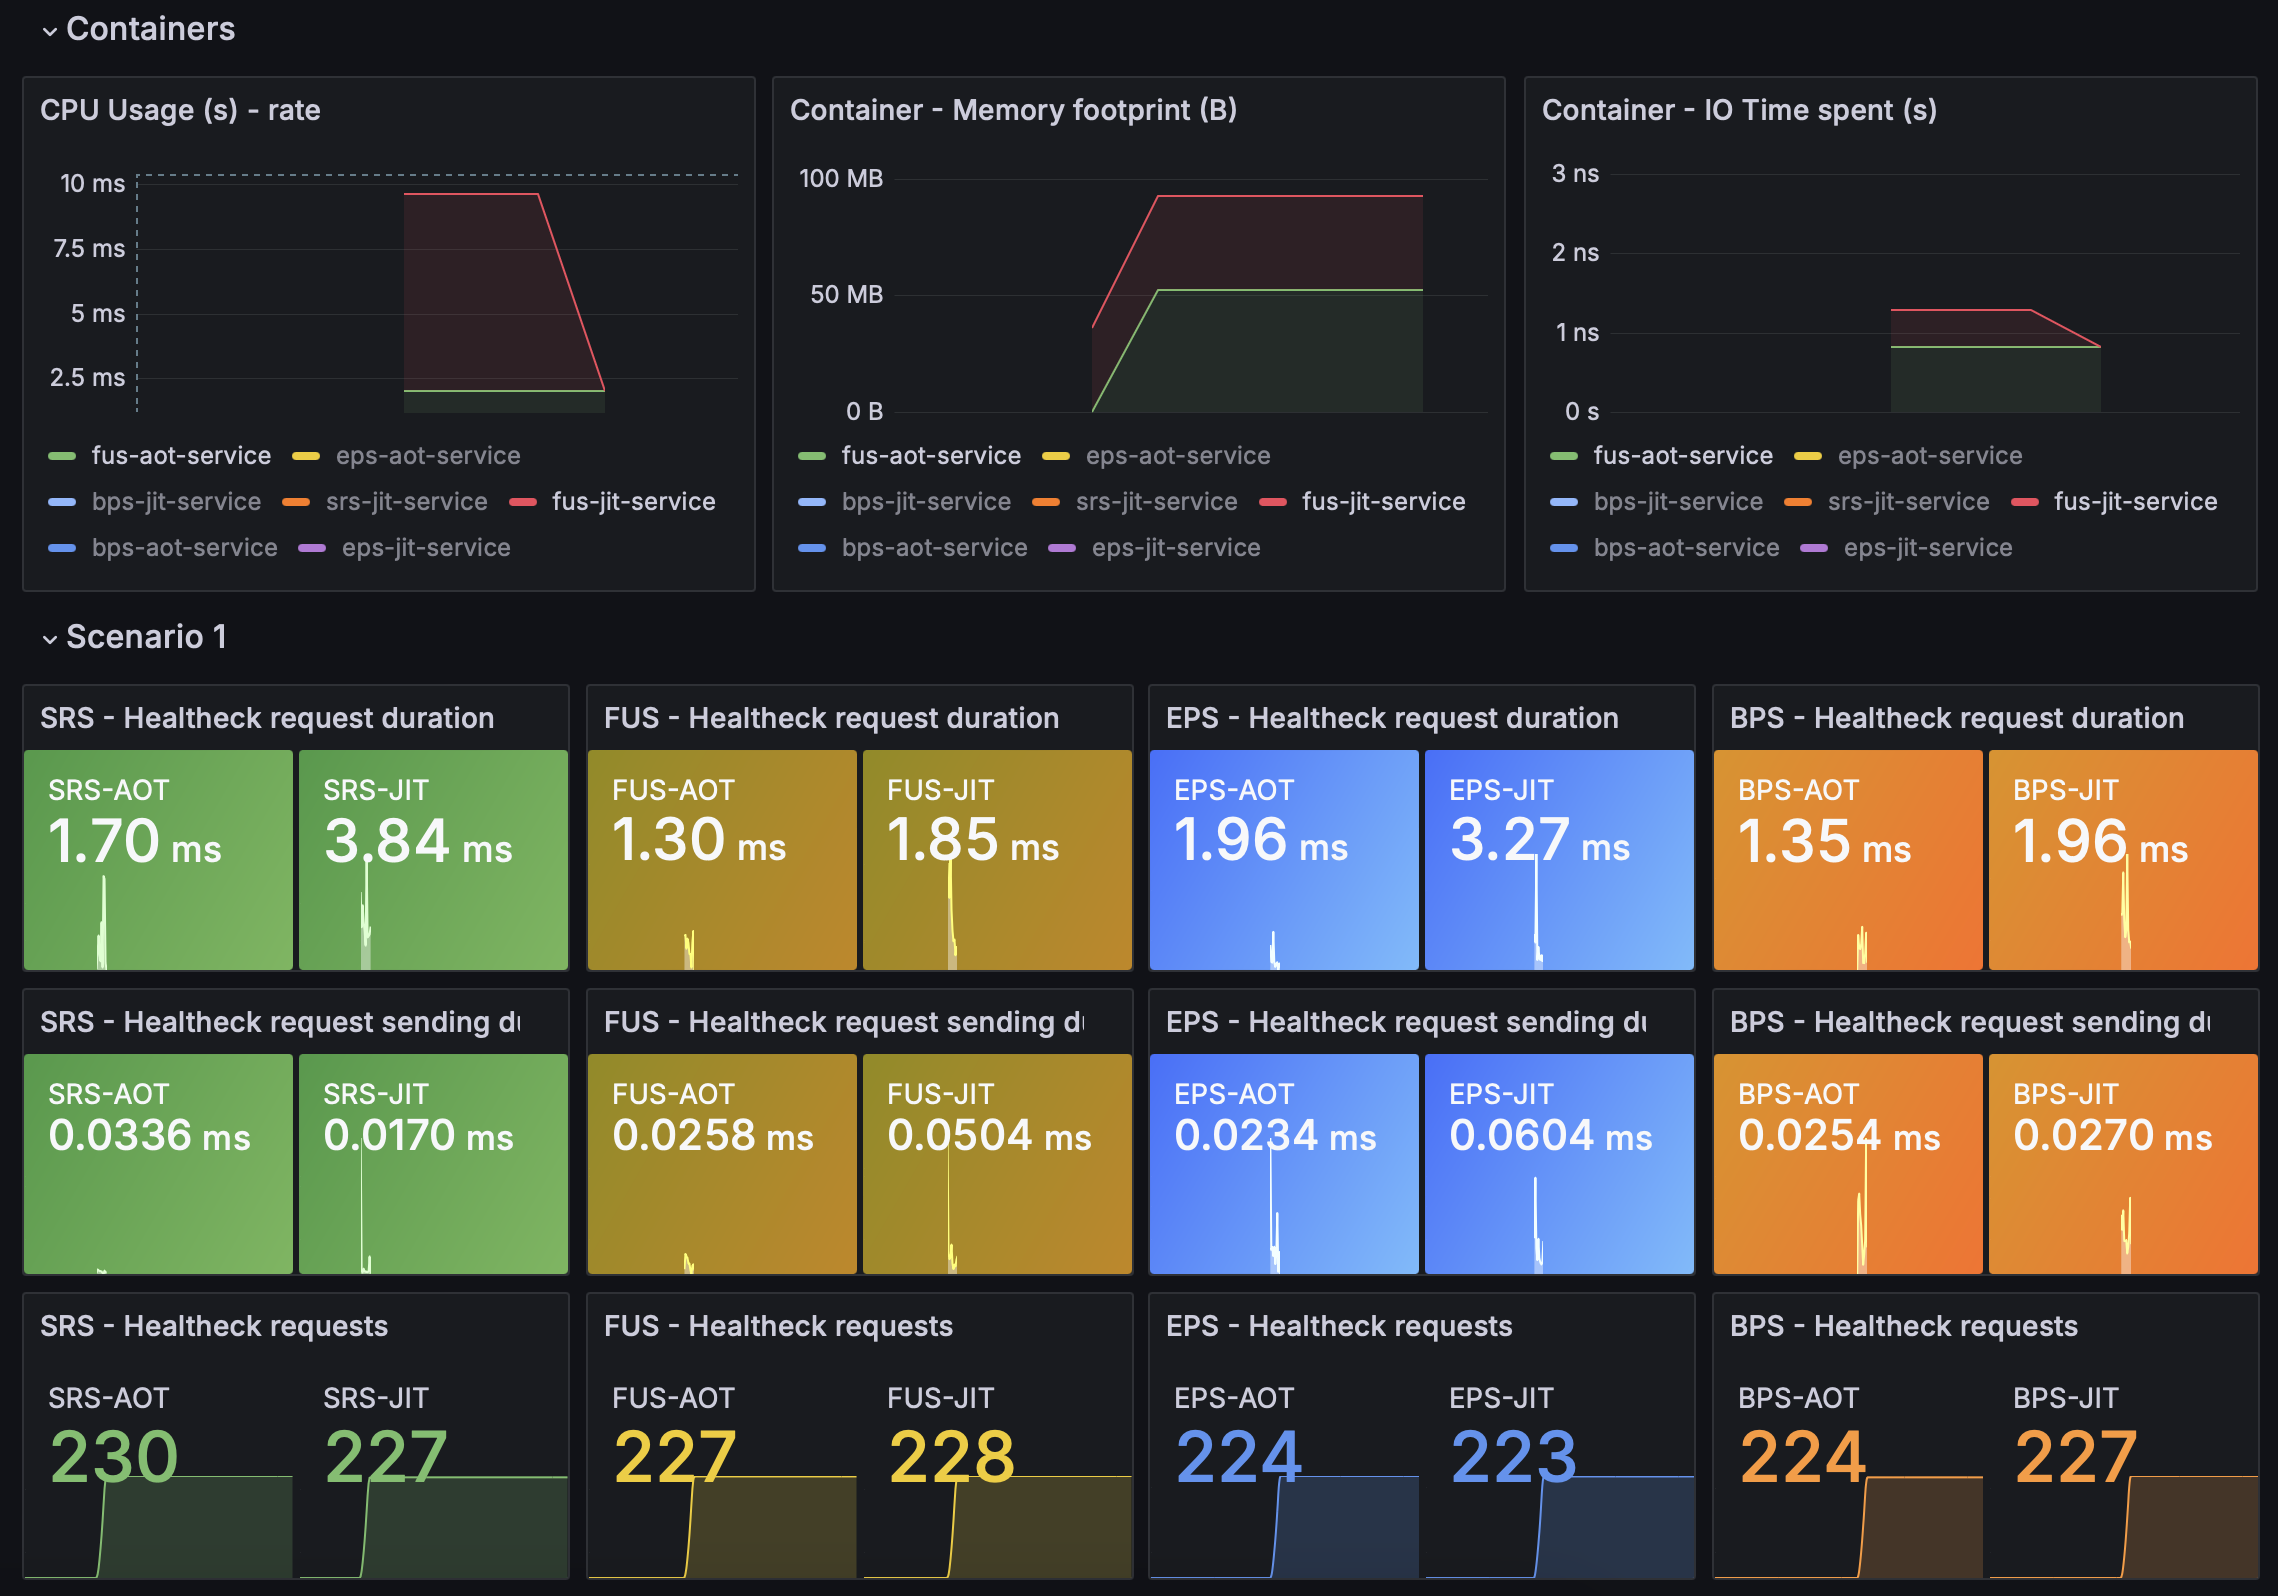
\includegraphics[width=1\textwidth]{graphics/images/scenario1-dashboard.png}
    \caption{Scénář 1 - Grafana dashboard}
    \label{fig:scenario1dashboard}
\end{figure}

% ============================================================================ %
 % Prilohy


% ============================================================================ %

\end{document}

% ============================================================================ %
